\subsection{Conditioning and reference matching resolve diversity reversals}
\label{sec:t2i}
We compare SD1.5, native LCM-LoRA,
one-step DMD2, and Sana-600M
\cite{rombach2022ldm,luo2023lcmlora,yin2024dmd2,xie2025sana} on 128 held-out
PartiPrompts~\cite{yu2022parti}, with eight diagnosis and 16 separate outcome
seeds per prompt. Disjoint pools supply 32 representation-fit, 256 calibration,
and 48 development prompts. The complete matrix retains 29 SD and seven
Sana configurations. References are DDIM50 at classifier-free guidance
(CFG) 7.5 and Flow-DPM++50;
DMD2 also uses its training-matched CFG1.75 teacher. These are generator-relative
measurements; prompts supply no real-image coverage target. The evaluated
configurations include step and guidance changes, stochastic sampling,
conditioning noise, and first-base-step LCM. Native schedules and checkpoint
conversions are checked against released implementations. Prompt-level
resampling keeps each prompt's candidate/reference pairing intact and treats
its seeds as within-prompt observations.

DDIM4 has pooled DINO spread ratio 0.919 [0.910,0.928], yet within-prompt
spread ratio 1.306 [1.236,1.382] (Fig.~\ref{fig:t2i_representations}).
A secondary descriptive decomposition, specified after access to these
outcomes, explains the reversal. Within-prompt variation rises from
0.400 to 0.523 of reference pooled spread, while the between-prompt
contribution falls from 0.600 to 0.396. The larger decrease pulls the
sum below one. The within-prompt ratio uses only the reference within
component. Sampling-latent and image-re-encoding
ratios are 0.414 and 0.482. The PickScore preference proxy
\cite{kirstain2023pickapic} is 0.247 [0.227,0.268],
below the frozen 0.45 tolerance, so fidelity qualifies the interpretation
of the increased feature spread.

\begin{figure}[t]
\centering
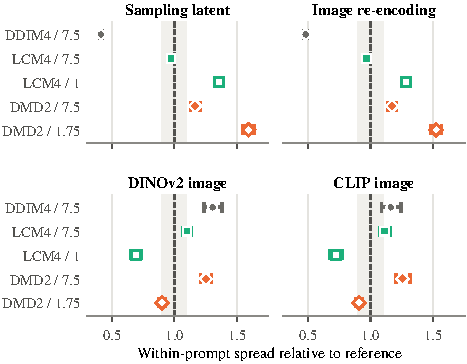
\includegraphics[width=\linewidth]{../figures/t2i_representation_reference.pdf}
\caption{Conditioning and reference matching change the measured direction.
Five comparisons, four representations: conditional trace ratios with
\emph{descriptive} 95\% paired prompt-bootstrap intervals. Rows give sampler
and teacher CFG; open markers indicate the alternate teacher. The band marks
$[0.9,1.1]$ and the dashed line marks equality. LCM CFG1 is a sensitivity;
DMD2 CFG1.75 is training-matched. The supplement retains the separate
simultaneous 20-contrast checks.}
\label{fig:t2i_representations}
\end{figure}

DMD2's DINO ratio changes from 1.251 [1.208,1.297] against CFG7.5 to
0.901 [0.873,0.929] against its matched CFG1.75 teacher. The latter is
below equality but unresolved at the 0.9 contraction margin. Against that
teacher, latent spread increases to 1.592 and learned preference reaches
0.558 [0.545,0.571]. LCM4's DINO ratio changes from 1.101 against CFG7.5
to 0.695 against CFG1; this external-guidance sensitivity is not a verified
training-matched teacher and fails CLIP support compatibility.

Sana Euler8 reduces latent spread to 0.763 [0.746,0.779] while DINO spread
rises to 1.118 [1.083,1.157]. At eight calls, Flow-DPM++ retains paired
learned preference within tolerance, 0.479 [0.471,0.487]. CADS increases
DINO spread to 1.965 [1.828,2.121] but lowers preference to
0.354 [0.339,0.369]. The same measurement discipline distinguishes added
variation from a fidelity-qualified improvement across these model families.
